\documentclass[a4paper,12pt,titlepage]{article}

\title{Unidade 3 - Banco de Dados}
\author{Fernando de Lima Gonçalves}
\date{Belo Horizonte \\ 10/2026}

\usepackage{graphicx}
\usepackage{titlesec}
\usepackage{xcolor}
\usepackage[portuguese]{babel}
\usepackage[colorlinks=true,allcolors=teal]{hyperref}

% Caminho de mídia
\graphicspath{{img/}}

% Cada tópico em página nova
\newcommand{\sectionbreak}{\clearpage}

\begin{document}

\maketitle

\tableofcontents

\section{Origem}
\begin{itemize}
    \item 
        Fortemente baseado na \textbf{Teoria dos Conjuntos}
    
    \item
        Banco de Dados como um conjunto de dados: \textbf{\textit{TABELAS}}

\end{itemize}

\begin{figure}[h]
    \centering
    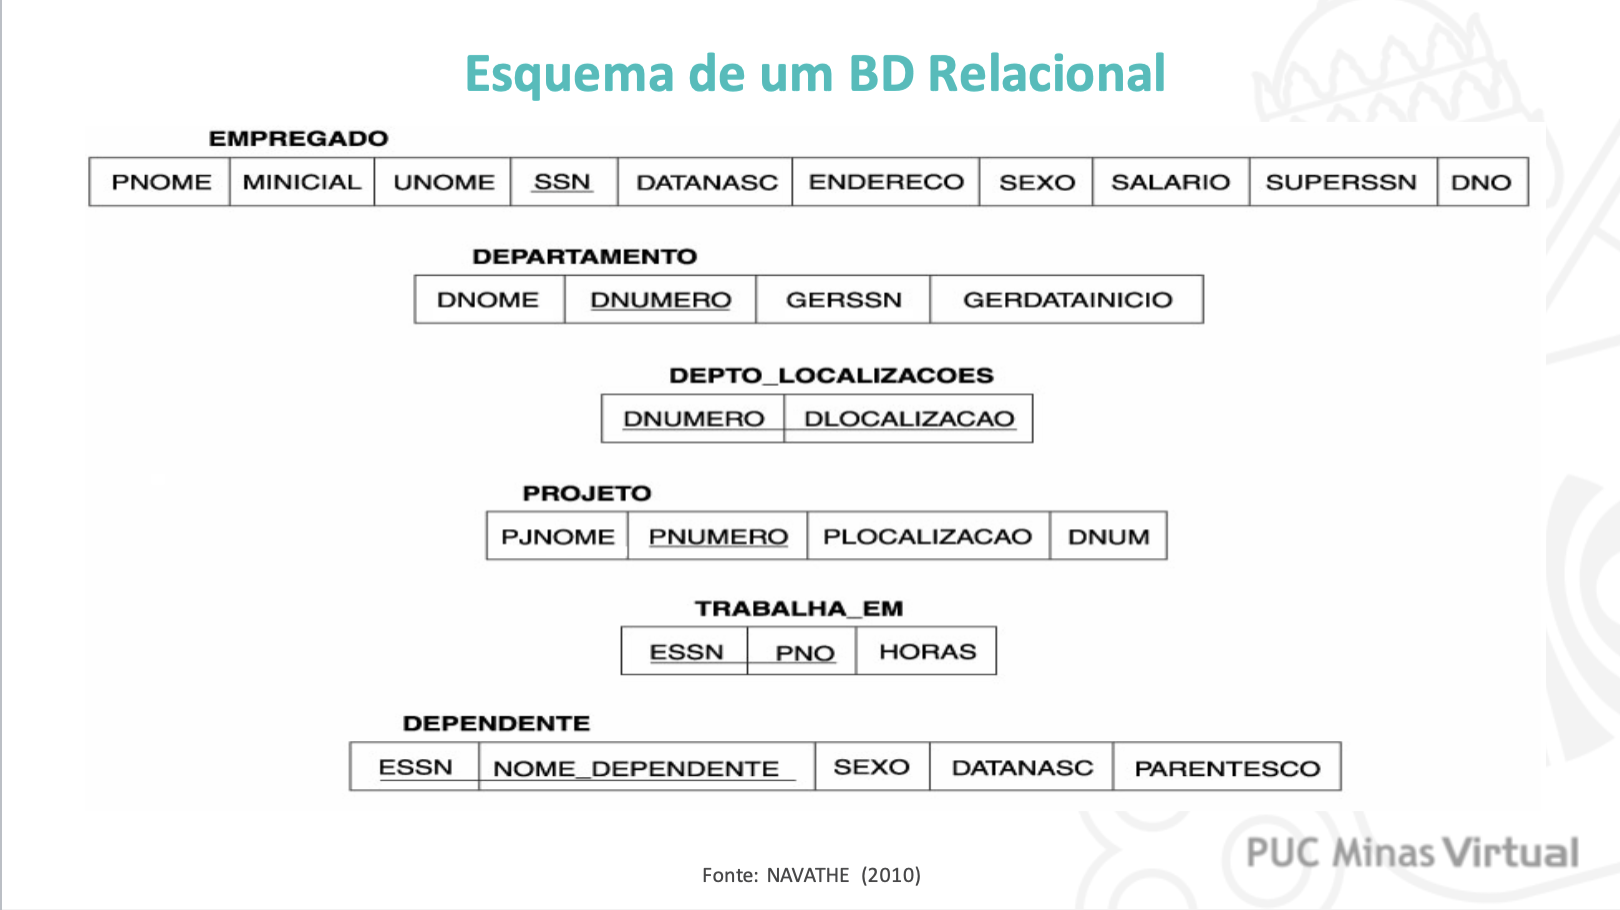
\includegraphics[scale=0.4]{u3_1.png}
    \label{fig:esquemas_bd-relacional}
    \caption{\footnotesize \textit{BARONI}, Rodrigo - Unidade 3.1: Modelo Relacional}
\end{figure}

\begin{figure}[h]
    \centering
    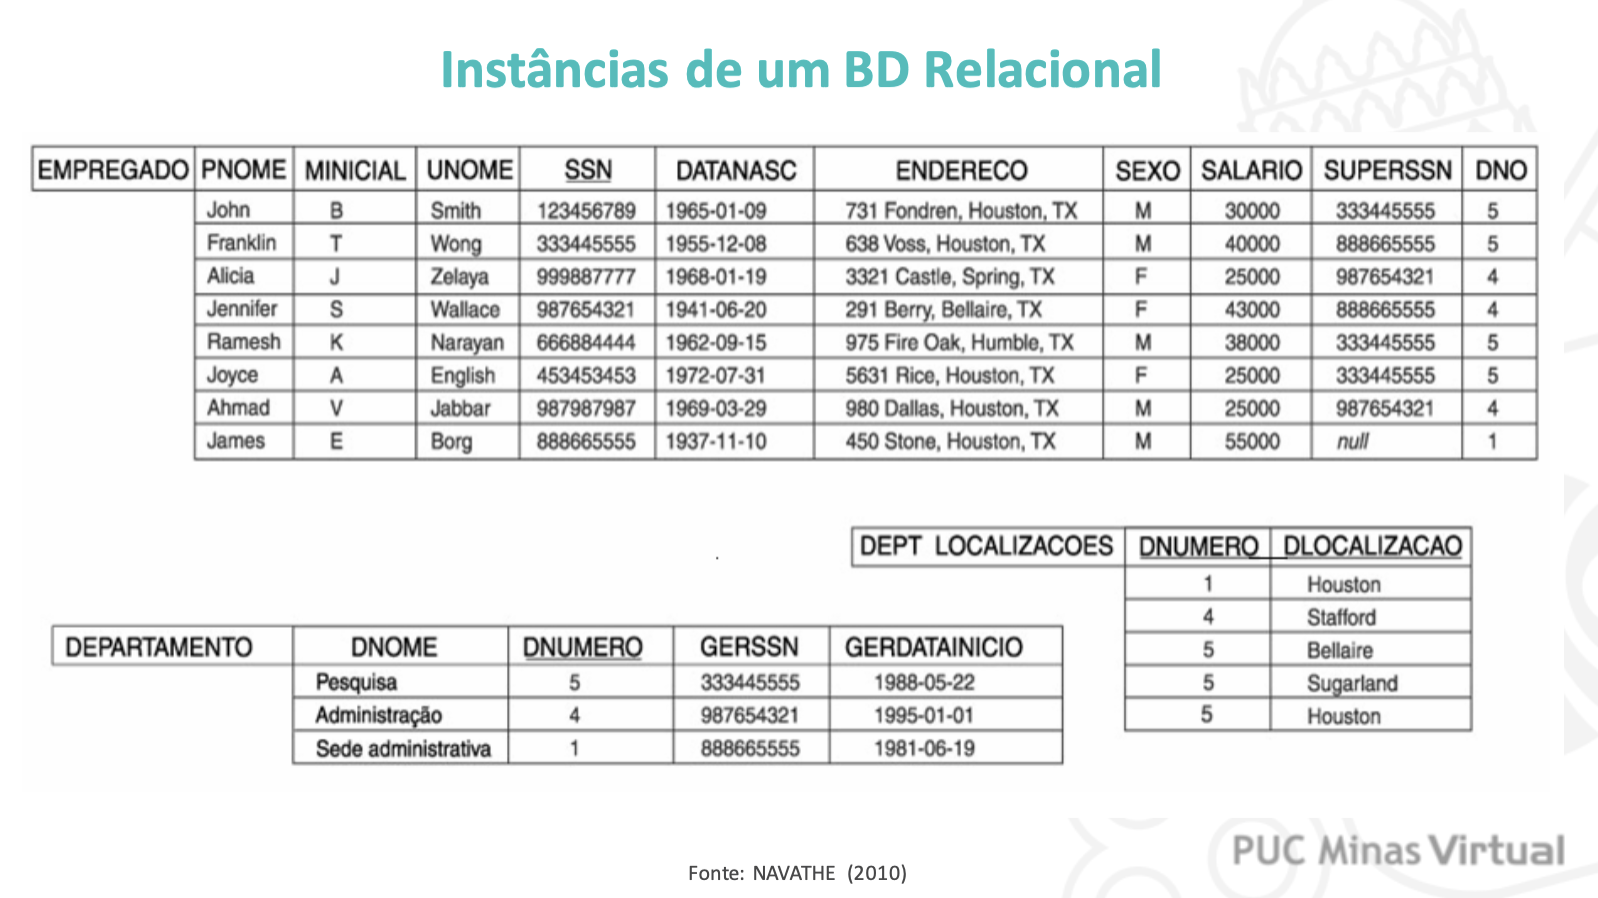
\includegraphics[scale=0.4]{u3_2.png}
    \label{fig:instancias_bd-relacional}
    \caption{\footnotesize \textit{BARONI}, Rodrigo - Unidade 3.1: Modelo Relacional}
\end{figure}

\section{Relação: Partes e Propriedades}

\end{document}
